\documentclass[10pt]{article}
\usepackage{a4wide}
\usepackage[english]{babel}
\usepackage{graphicx}
\usepackage{tabu}
\usepackage{textcomp}
\usepackage{fancyhdr}
\usepackage{lastpage}
\usepackage{titlesec}
\usepackage{lscape}
\usepackage{longtable}
\usepackage{color}
\usepackage{listings}
\usepackage{xkeyval}
\usepackage{hyperref}
\usepackage[utf8]{inputenc}
\usepackage{amsmath}

\definecolor{mygreen}{rgb}{0,0.6,0}
\definecolor{mygray}{rgb}{0.5,0.5,0.5}
\definecolor{mymauve}{rgb}{0.58,0,0.82}

\lstset{ % Syntax highliughting for java
  backgroundcolor=\color{white},   % choose the background color; you must add \usepackage{color} or \usepackage{xcolor}
  basicstyle=\footnotesize,        % the size of the fonts that are used for the code
  breakatwhitespace=false,         % sets if automatic breaks should only happen at whitespace
  breaklines=true,                 % sets automatic line breaking
  captionpos=b,                    % sets the caption-position to bottom
  commentstyle=\color{mygreen},    % comment style
  deletekeywords={...},            % if you want to delete keywords from the given language
  escapeinside={\%*}{*)},          % if you want to add LaTeX within your code
  extendedchars=true,              % lets you use non-ASCII characters; for 8-bits encodings only, does not work with UTF-8
  frame=none,                    % adds a frame around the code
  keepspaces=true,                 % keeps spaces in text, useful for keeping indentation of code (possibly needs columns=flexible)
  keywordstyle=\color{blue},       % keyword style
  language=Octave,                 % the language of the code
  morekeywords={*,...},            % if you want to add more keywords to the set
  numbers=left,                    % where to put the line-numbers; possible values are (none, left, right)
  numbersep=5pt,                   % how far the line-numbers are from the code
  numberstyle=\tiny\color{mygray}, % the style that is used for the line-numbers
  rulecolor=\color{black},         % if not set, the frame-color may be changed on line-breaks within not-black text (e.g. comments (green here))
  showspaces=false,                % show spaces everywhere adding particular underscores; it overrides 'showstringspaces'
  showstringspaces=false,          % underline spaces within strings only
  showtabs=false,                  % show tabs within strings adding particular underscores
  stepnumber=5,                    % the step between two line-numbers. If it's 1, each line will be numbered
  stringstyle=\color{mymauve},     % string literal style
  tabsize=4,                       % sets default tabsize to 2 spaces
  title=\lstname                   % show the filename of files included with \lstinputlisting; also try caption instead of title
}
%%%%%%
%% Variables for version and release status
%% useage: \version
%%%%%%
\newcommand\module{CS36110}
\newcommand\assignmentTitle{Machine Learning Assignment 1}
\newcommand\authorText{Nicholas Dart}
\newcommand\authorUsername{nid21}
\newcommand\studentID{130057750}
\newcommand\assesser{Neil Mac Parthaláin}

%%%%%%
%% Alias
%%%%%%
%\newcommand{\sectionbreak}{\clearpage}    %% Allways start a section on a new page

\title{ \huge \module~Assignment \\ \Large \assignmentTitle}
\author{
  \vspace{100pt}
  \begin{tabular}{ r || l }
    Author          & \authorText (\authorUsername)\\
            & \studentID \\
    Date Published  & \today \\
            & \\
    Assessed By     & \assesser \\
    Department      & Computer Science \\
    Address         & Aberystwyth University \\
            & Penglais Campas \\
            & Ceredigion \\
            & SY23 3DB \\
  \end{tabular} \\
  Copyright \textcopyright~Aberystwyth University 2015
  %get rid of the date on the titlepage
  \date{}
}

\pagestyle{fancy}
\fancyhf{}
\lhead{\module~Assignment}
\rhead{\authorText~-~\studentID}
\rfoot{Page \thepage \hspace{1pt} of \pageref{LastPage}}
\lfoot{Aberystwyth University - Computer Science}

\begin{document}
  \setcounter{page}{1}

  % \maketitle
  % \thispagestyle{empty}
  % \clearpage

  % \tableofcontents
  % \clearpage

  \section{Classifiers}

    \subsection{Naïve Bayse}
      \label{sec:bayseInitialTraining}

      Naïve Bayse broadly refers to a collection of classification algorithm based on Bayse theorem, and rely on the probably naïve assumption that all attributes or features are independent of each other (hence where the name comes from). Bayse theorem is is defined as;

      \begin{equation*}
        P\left(H|D\right) = \frac{P\left(D|H\right) P\left(H\right)}{P\left(D\right)}
      \end{equation*}

      This theorem can be used for multiple pieces of data, or ``features'' by multiplying the resultant probabilities together. Hence we get a simple Naïve Bayse classifier:

      \begin{equation*}
        P\left(h|Multiple Data\right) = P\left(a_1,a_2...a_n | v_j\right) = \prod_{i}{P\left(a_i,|v_j\right)}
      \end{equation*}

      Naïve Bayse is a very simple classifier that requires relatively little computation, hence it is very fast. As a result of this, it can also be trivially retrained with future data very easily, making it ideal for real world applications. Applications of Naïve Bayse include spam detection, object classification and filtering. The caveat of Naïve Bayse is implied by it's name; it is ``naïve''. It does not take into account any relations between features which often have relations to other features. \\

    \subsection{C4.5 Decision Tree}
      \label{sec:j48InitialTraining}

      C4.5 is a decision tree generating algorithm developed by Ross Quinlan, derived from the earlier ID3 algorithm by the same author, that is used for classification. C4.5 and ID3 (and J48, a Java implementation of C4.5) use concepts from entropy and information theory to determine how to build the tree. C4.5 unlike it's predecesor ID3 can deal with continuous data sets\cite{quinlan_c4.5_improved} and missing feature values. 

      C4.5 build decision trees by determining the most important features using entropy theory and information gain. The feature with the highest score is chosen first, and then it's values are added as leafes. The process is repeated for each child leaf until it is said to be ``pure'', that is the leaf has an entropy of 0.

      \begin{equation*}
        Entropy(S) \equiv
          \sum^{c}_{i=1}p_i log_2 \left(\frac{1}{p_i}\right) =
          \sum^{c}_{i=1}-p_1 log_2 \left(p_i\right)
      \end{equation*}

      \begin{equation*}
        Gain\left(S, A\right) = Entropy\left(S\right) - \sum_{v \in Value\left(A\right)} \frac{|S_v|}{|S|}Entropy\left(S_v\right)
      \end{equation*}

      C4.5 is a rather robust tool that can deal with noisy or missing data, through a number of means \cite{quinlan_c4.5}, can deal with real natural numbers (ID3 cannot work with real). It also has the advantage that the output is a relatively simple graph which can be traversed by hand and understood easily. C4.5 however is not well suited to problems with XOR components (one, the other, but not both) as the tree can grow very large.

      As with any machine learning tool, there exists the possibility of overfitting or overtraining the algorithm, such that it better or perfectly classifies the training data but performed worse in a general/live case. This is said to have happened when a trained algorithm is better at predicting known data but worse at predicting new data. \\

  \section{Configurations}

    During the course of using WEKA, J48 and Naïve Bayse were both used with 5-fold cross validation and the default seed provided by WEKA (v3.6.10)

    \subsection{Missing Values}
      The Weka library provides a utility to replace missing attribute values with either the mean of the feature for numeric data, or the mode for nominal data. The latter approach of replacing nominal data with the mode is relatively sensible; a mean is not appropriate.

      Replacing numeric data with the mean however could mislead the algorithms as rather than the algorithm deciding what should be done, the lack of information is covered up. Doing this will however result in all the available data being usable for algorithms that do not support empty attributes.

      Running the replaceMissingValues filter replaces four values in attribute 12 (NumOfMajorVesselsFlouroscopy) and two values in attribute 13 (Thal.)\\

    \subsection{Binarising Result Field}
      This was achieved with a simple regex replace (\texttt{/([1-5])\$/} matches replaced with \texttt{1}) and changing the nominal set from \texttt{\{0-4\} to \{0-1\}}.

    \subsection{Naïve Bayse}

      %%% From WEKA:
      %
      % SYNOPSIS
      % Class for a Naive Bayes classifier using estimator classes. Numeric estimator precision values are chosen based on analysis of the  training data. For this reason, the classifier is not an UpdateableClassifier (which in typical usage are initialized with zero training instances) -- if you need the UpdateableClassifier functionality, use the NaiveBayesUpdateable classifier. The NaiveBayesUpdateable classifier will  use a default precision of 0.1 for numeric attributes when buildClassifier is called with zero training instances.
      %
      % For more information on Naive Bayes classifiers, see
      %
      % George H. John, Pat Langley: Estimating Continuous Distributions in Bayesian Classifiers. In: Eleventh Conference on Uncertainty in Artificial Intelligence, San Mateo, 338-345, 1995.
      %
      % OPTIONS
      % debug -- If set to true, classifier may output additional info to the console.
      %
      % displayModelInOldFormat -- Use old format for model output. The old format is better when there are many class values. The new format is better when there are fewer classes and many attributes.
      %
      % useKernelEstimator -- Use a kernel estimator for numeric attributes rather than a normal distribution.
      %
      % useSupervisedDiscretization -- Use supervised discretization to convert numeric attributes to nominal ones.

      Weka provides two additional options to choose when running Naïve Bayse; \texttt{kernel estimator} and \texttt{supervised discretization}. The Kernel (density) Estimator is used as an alternative to a normal distribution\cite{kernelEstimator}. The Supervised Discretization option is used to convert real or numeric data to nominal data\cite{discretizeFilter}. \\

    \subsection{J48}

      %%% From WEKA:
      % SYNOPSIS
      % Class for generating a pruned or unpruned C4.5 decision tree. For more information, see
      %
      % Ross Quinlan (1993). C4.5: Programs for Machine Learning. Morgan Kaufmann Publishers, San Mateo, CA.
      %
      % OPTIONS
      % binarySplits -- Whether to use binary splits on nominal attributes when building the trees.
      %
      % confidenceFactor -- The confidence factor used for pruning (smaller values incur more pruning).
      %
      % debug -- If set to true, classifier may output additional info to the console.
      %
      % minNumObj -- The minimum number of instances per leaf.
      %
      % numFolds -- Determines the amount of data used for reduced-error pruning.  One fold is used for pruning, the rest for growing the tree.
      %
      % reducedErrorPruning -- Whether reduced-error pruning is used instead of C.4.5 pruning.
      %
      % saveInstanceData -- Whether to save the training data for visualization.
      %
      % seed -- The seed used for randomizing the data when reduced-error pruning is used.
      %
      % subtreeRaising -- Whether to consider the subtree raising operation when pruning.
      %
      % unpruned -- Whether pruning is performed.
      %
      % useLaplace -- Whether counts at leaves are smoothed based on Laplace.

      For J48 WEKA provides a number of additional options; \texttt{binarySplits}, \texttt{confidenceFactor}, \texttt{minNumObj}, \texttt{numFolds}, \texttt{reducedErrorPruning}, \texttt{saveInstanceData}, \texttt{subtreeRaising}, \texttt{unpruned}, and \texttt{useLapse}. Experimenting with various options, only with reducedErrorPrungin set to True was the accuracy of classification reduced. 

      Reduced error pruning is a process by removing or compressing a node and it's children (thus turning it to a leaf node) with the goal of improves the accuracy of the classification and reducing any effects of overtraining the algorithm. It also has the added benefit of reducing the size of the tree which will help in human readability.

  \section{Results}

    The table of results below shows percentage correctly identified results for both J48 and Naïve Bayse, as well as the size of tree for J48.\\

    {
      \centering
      \begin{tabular}{ | r || c || c | c | c |}
        \hline
        {}                              & \textbf{Naïve Bayse}                        & \multicolumn{3}{c |}{\textbf{J48}} \\ \hline
        {}                              & Correctly Classified & Correctly Classified & Leaves in Tree & Size of Tree \\ \hline
        Raw Cleveland Data              & 55.4455 \%           & 51.8152 \%           & 34             & 67 \\ \hline
        Cleveland Data Missing Replaced & 55.4455 \%           & 52.4752 \%           & 32             & 63 \\ \hline
        Binarized Without Missing       & 83.4983 \%           & 77.8878 \%           & 17             & 33 \\ \hline
        J48 Reduced Error Pruning       & N/A                  & 79.8680 \%           & 9              & 15 \\ \hline
      \end{tabular}
    }

    The initial classification attempt with unaltered data yielded aproximatly \textbf{50\%} for both Bayes and J48, this included both algorithms working with a total of six missing feature values. At this level of accuracy I would not call either approach better than the other, as in only half of the cases would a result be correct. This result would be further worsened by the presence of false positives and false negatives, where a patient is diagnosed with having the disease when really they don't, or vice-versa.

    % False positives/False Negatives?

    Cleaning the input data of missing values by replacing them with the means and modes yields no change to Bayes, likely due to how it internally deals with missing values. J48 however produces a small (\texttt{+0.66\%}) increase for J48. I would not say this is a significant enough improvement to conclude that replacing values with their means is the correct course. Looking at the data it would make sense if the values that were replaced were whole numbers (the mean of all of the effected values were not whole), changing the field types from numeric to nominal may make sense, or further filtering the values to round them.

    Binarising the output values (feature 14, Num) and maintaining the replacement of missing values yielded a further improvement to both Bayse and J48 of \texttt{+28.0528\%} and \texttt{+26.0726\%} respectively. This increase is not surprising to me as the resulting values are simply compressed. In the previous classification attempts, it is considered incorrect if a value of \textbf{4} is produces instead of \textbf{3}, whereas after here that would be considered correct. Nevertheless it is a significant improvement to both. This step also reduces the size of the decision tree produced. Such outputs would likely be more valuable to medical professionals who have limited time and so would desire an easier chart or process to follow.

    Applying the reduced error pruning in J48 nearly brings it to par wit h Bayse, however produces a significantly smaller tree. (see figure \ref{fig:j48ReducedErrorPruning})

    \begin{figure}
      \centering
      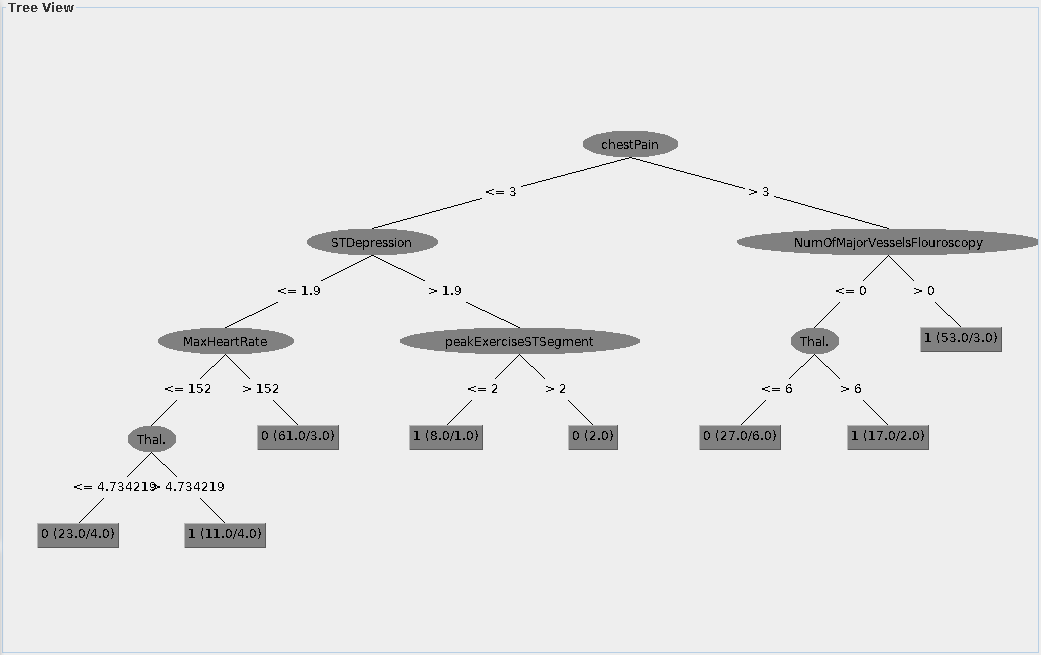
\includegraphics[width=0.8\textwidth]{./j48-pruned-tree.png}
      \caption{J48 with Reduced error pruning.}
      \label{fig:j48ReducedErrorPruning}
    \end{figure}

  \begin{thebibliography}{9}
      \bibitem{quinlan_c4.5_improved} 
        J. R. Quinlan: Improved use of continuous attributes in c4.5 (accessed 04/11/16),\\
        \url{https://www.jair.org/media/279/live-279-1538-jair.pdf}

      \bibitem{quinlan_c4.5}
        J. R. Quinlan: C4.5: Programs for Machine Learning (accessed 04/11/16),\\
        \url{http://link.springer.com/article/10.1007/BF00993309}

      \bibitem{kernelEstimator}
        University of Waikato, Hamilton, New Zealand (accessed 08/11/16)
        \url{https://github.com/bnjmn/weka/blob/8bc715f1d72bf43e1b3c7a1b5ca7a792a4a7cde0/weka/src/main/java/weka/estimators/KernelEstimator.java}

      \bibitem{discretizeFilter}
        University of Waikato, Hamilton, New Zealand (accessed 08/11/16)
        \url{https://github.com/bnjmn/weka/blob/24a72d94fefeb4e6ba4172e63db9b8c52c3850d1/weka/src/main/java/weka/filters/supervised/attribute/Discretize.java}
  \end{thebibliography}

\end{document}